\chapter{Design of a Fault Detection and Diagnosis System for Photovoltaic Systems}
\label{ch:conception}

\section{Introduction}

The process of designing a FDD system for photovoltaic systems involves several parts, including system architecture, dataset selection, data preprocessing, feature engineering, model selection and evaluation.
Each of these steps is cruicial to build a robust and effective FDD solution. The following sections will detail the design choices made for each step.

\section{System Architecture}
The overall architecture includes 4 main components, as illustrated in figure \ref{fig:system_architecture}:
\par\noindent\textbf{Data collection and transformation:} Collects raw data from sensors such as irradianceand ambient temperature, and electrical signals and applies the necessary preprocessing and transformations
to make it suitable for input to the next stage of the system.
\par\noindent\textbf{Anomaly Detection:} Upon receiving the preprocessed data, this component detects persistent deviations from expected values under observed meteorological conditions. Such deviations may indicate an anomaly in the system.
\par\noindent\textbf{Fault Diagnosis:} If an anomalt is detected, this component's responsability is to determine the type of fault that has occured from a pre-determined set of faults.
\par\noindent\textbf{Monitoring Interface:} Displays the system's real-time status, including detected anomalies, diagnosed faults along with their confidance scores, incoming data visualizations and performance rapports. 


\begin{figure}[H]
    \centering
    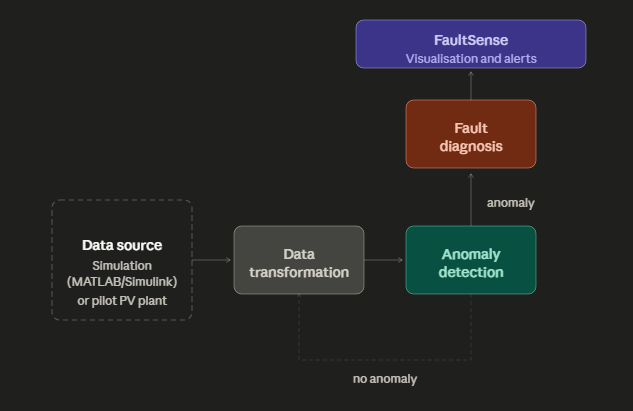
\includegraphics[width=0.8\textwidth]{figures/chap3/fdd-arch.png}
    \caption{FDD System Architecture.}
    \label{fig:system_architecture}
\end{figure}

\section{Dataset Selection}
Based on the previous dataset survey in\ref{sec:data-survey}, the Costa and La Réunion datasets were selected for the development and evaluation of our FDD system.
\textbf{Costa} is the primary experimental dataset, collected from a grid-connected pilot PV plant located in City of Curitiba-State of Paraná, Brazil. It contains 16 Canadian 330W Poly-crystalline Modules (CS6U-330P) divided into 2 strings of 8 modules each
running the Maximum Power Poin Tracking (MPPT) algorithm. The system may yeild 5kW peak installed capacity \citep{MonitoringSystemOnline2020}. The figure \ref{fig:costa_circuit} illustrates in detail the electrical configuration.
\begin{figure}[H]
    \centering
    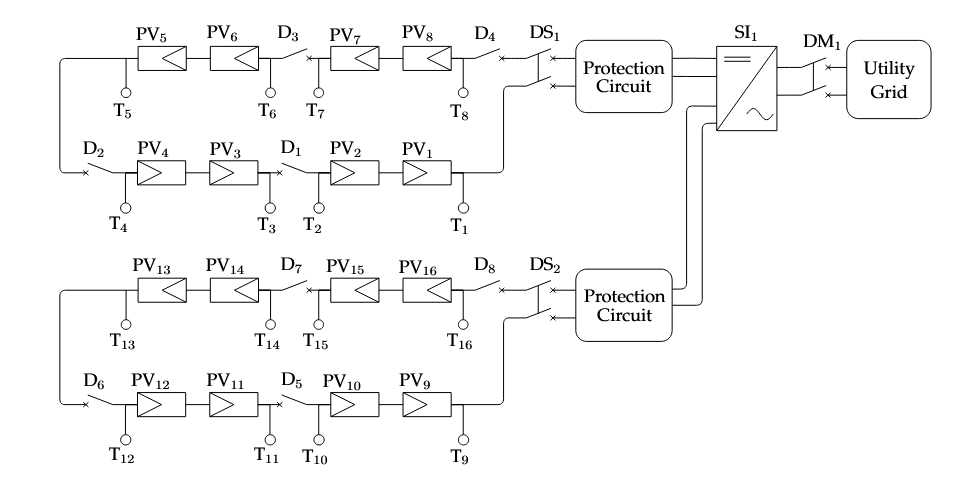
\includegraphics[width=0.8\textwidth]{figures/chap3/costa-shema.png}
    \caption{Costa Photovoltaic Plant Electrical Diagram \citep{MonitoringSystemOnline2020}.}
    \label{fig:costa_circuit}
\end{figure}

This dataset contains 4 fault types: \textbf{Shadowing}, \textbf{Degradation}, \textbf{Open-Circuit} and \textbf{Short-Circuit}. The full detail is illustrated in Table~\ref{tab:costa_label_counts}.

\begin{table}[H]
    \centering
    \caption{Number of data points in the Costa dataset.}
    \label{tab:costa_label_counts}
    \begin{tabular}{l r}
        \toprule
        Label & Number of data points \\
        \midrule
        Degradation & 10,371 \\
        Short-circuit & 5,999 \\
        Open-circuit & 6,024 \\
        Partial shadowing & 184,311 \\
        No fault introduced & 309,253 \\
        \midrule
        Total & 515,958 \\
        \bottomrule
    \end{tabular}
\end{table}

This dataset was chosen for its real-world nature which captures the noise and imperfections of actual PV system measurements, as well as its diverse fault types
and the presence of a large number of data points which allows for robust model training and evaluation. Additionally, the dataset includes both electrical and meteorological measurements. A full list of available features is provided in Table~\ref{tab:costa_features}.

\begin{table}[H]
    \centering
    \caption{Costa dataset features and descriptions.}
    \label{tab:costa_features}
    \begin{tabularx}{\textwidth}{l X}
        \toprule
        Feature & Description \\
        \midrule
        \texttt{vdc1} & voltage measured for string~1 (V). \\
        \texttt{vdc2} & voltage measured for string~2 (V). \\
        \texttt{idc1} & current measured for string~1 (A). \\
        \texttt{idc2} & current measured for string~2 (A). \\
        \texttt{pdc1} & power measured for string~1 (W). \\
        \texttt{pdc2} & power measured for string~2 (W). \\
        \texttt{pdc} & total power measured for the system (W). \\
        \texttt{pvt} & Average PV module temperature (\textdegree{}C). \\
        \texttt{irr} & Solar irradiance (W/m$^2$). \\
        \bottomrule
    \end{tabularx}
\end{table}

\textbf{La Réunion} dataset is collected from a 4 kW rooftop photovoltaic installation located on the campus of the University of La Réunion, Saint-Denis, La Réunion Island, Indian
Ocean\citep{graillet2023dib}. The plant comprises 2 inverter lines, each consisting of 12 polycrystalline modules arranged as 2 parallel series of 6 panels, mounted at a tilt angle of 26°. The inverter line on which faults are 
induced (line~1) operates alongside a second line (line~2) kept in normal conditions throughout the experiments, providing a contemporaneous control reference under identical irradiance. Electrical production data is acquired per inverter line through an Energrid datalogger at 0.2~Hz (one sample every 5~seconds). Meteorological quantities (global and diffuse tilted irradiance GTI and DTI [W~m$^{-2}$], and module back-surface temperature $T_{\mathrm{PV}}$ [°C]) are recorded at 1~Hz via a Campbell Scientific CR1000X datalogger equipped with a Delta-T Devices SPN1 pyranometer and type-T and type-K thermocouples. Data are transmitted over TCP/IP and stored in an InfluxDB time-series database; the dataset spans October~2021 to April~2023, totalling 2\,988\,814 samples \citep{graillet2023dib}.
Fault conditions correspond exclusively to shading variants, each induced by applying
an opaque mask to the relevant modules: uniform shading of the entire line (label 1),
constant partial shading of 1 to 3 complete modules (labels 2.1–2.3), constant partial
shading of fractions of a single module (labels 3.1–3.2), and static intermittent partial
shading produced by a fixed shadow-casting object (label 4). The fault type is recorded
as a numeric variable directly in the database at the time of induction. Because all fault
conditions involve some form of irradiance reduction rather than an electrical integrity
change, the La Réunion fault taxonomy is structurally narrower than Costa’s. This
difference motivates its role as a pipeline generalization benchmark rather than as a
primary classification dataset. A full list of available features and fault types is provided in Table~\ref{tab:reunion-vars}.

\begin{table}[H]
\centering
\caption{La Réunion dataset: recorded variables and fault label encoding.}
\label{tab:reunion-vars}
\begin{tabular}{l p{7.5cm} c}
\toprule
\textbf{Column} & \textbf{Description} & \textbf{Unit} \\
\midrule
\texttt{Ia}    & Inverter AC current & A \\
\texttt{Ig}    & Grid AC current & A \\
\texttt{Va}    & Inverter AC voltage & V \\
\texttt{Vg}    & Grid AC voltage & V \\
\texttt{Pg}    & Grid AC power & W \\
\texttt{Eg}    & Energy injected to grid & kWh \\
\texttt{Fg}    & Grid frequency & Hz \\
\texttt{GTI}   & Global tilted irradiance & W~m$^{-2}$ \\
\texttt{DTI}   & Diffuse tilted irradiance & W~m$^{-2}$ \\
\texttt{TA}    & Ambient air temperature & $^\circ$C \\
\texttt{TPV}   & PV module back-surface temperature & $^\circ$C \\
\texttt{label} & Fault class: 0 Normal; 1 Uniform shading; 2.1--2.3 Constant partial shading (1--3 modules); 3.1--3.2 Partial module fraction; 4 Intermittent shading & -- \\
\bottomrule
\end{tabular}
\end{table}


% ────────────────────────────────────────────────────────────
\section{Exploratory Data Analysis}
\label{sec:eda}
% ────────────────────────────────────────────────────────────

The exploratory data analysis was structured as an 11-check audit applied independently to both field datasets before any modeling decision was made. Each check follows the same protocol: define the check, run it, record the finding, and record the explicit downstream consequence for the preprocessing or feature engineering described in Sections~\ref{sec:preprocessing} and~\ref{sec:feature-engineering}. This traceable structure is the basis for claiming that every pipeline design choice is data-driven rather than assumed.

\textbf{Schema validation and basic statistics.} The first check confirmed data types, row counts, and channel completeness. Costa yields 515,958 daytime rows across 16 recording days over 9 sensor channels (\texttt{vdc1}, \texttt{vdc2}, \texttt{idc1}, \texttt{idc2}, \texttt{pdc1}, \texttt{pdc2}, \texttt{pdc}, \texttt{irr}, \texttt{pvt}), with 0 missing values after ingestion-time irradiance trimming. La~Réunion yields 2,988,808 rows over a 19-month recording period across 9 channels (\texttt{Pg}, \texttt{Vg}, \texttt{Ig}, \texttt{Eg}, \texttt{Fg}, \texttt{Ia}, \texttt{GTI}, \texttt{TA}, \texttt{TPV}). Both datasets expose all labeled classes without gaps in the label column.

\textbf{Temporal coverage and sampling regularity.} The distribution of consecutive timestamp differences was computed over the full recording; gaps were catalogued at thresholds of 30\,s, 60\,s, and 300\,s. Figures~\ref{fig:eda-sampling-costa} and~\ref{fig:eda-sampling-reunion} show the distributions for both datasets. For Costa, p50 = p90 = p99 = 1.0\,s: the recording is a near-perfect 1~Hz sequence. Among all 515,942 consecutive pairs that fall within the same calendar day, only 20 exceed 30~s. For La~Réunion, intervals concentrate at 6~s (the dominant mode, $\approx$\,2.1 million occurrences) with a secondary cluster near 8~s; across the full 19-month recording, 528 consecutive pairs exceed 30~s with a tail that extends to multi-hour outages. This asymmetry is the primary driver of the dataset-specific imputation policies in Section~\ref{sec:preprocessing}; the 300-second gap threshold used for episode segmentation in Section~\ref{sec:splitting} was set from this distribution.

% \begin{figure}[H]
%   \centering
%   
\includegraphics[width=0.8\textwidth]{eda/costa_sampling_intervals.png}
%   \caption{Sampling interval distributions for Costa. Left: histogram zoomed to the 0.6--1.4\,s range, showing a single spike at 1\,s. Right: the complete interval distribution on a log-count axis, exposing the rare gaps above 30\,s.}
%   \label{fig:eda-sampling-costa}
% \end{figure}

\begin{figure}[H]
  \centering
  
\includegraphics[width=0.8\textwidth]{eda/reunion_sampling_intervals.png}
  \caption{Sampling interval distributions for La~Réunion. Left: intervals up to 30\,s; the dominant mode is 6\,s. Right: frequency of gaps exceeding 1\,minute (x-axis in hours), with 528 such events across the 19-month recording.}
  \label{fig:eda-sampling-reunion}
\end{figure}

\textbf{Missing value analysis.} A field time series can exhibit 3 structurally distinct missingness regimes: Missing Completely At Random (MCAR), where absent values are independent of all observed and unobserved variables; Missing At Random (MAR), where the probability of missingness depends on observed variables; and Missing Not At Random (MNAR), where it depends on the missing value itself. The distinction matters because MCAR and MAR permit principled imputation, while MNAR invalidates it. The null-value share was computed per column and per calendar day, and temporal clustering was assessed to assign each dataset to one of these regimes. For Costa, the irradiance-filtered ingestion frame contains 0 missing values across all 9 channels; the question does not arise. For La~Réunion, Figure~\ref{fig:eda-nulls} shows that missingness in the meteorological channels is sharply concentrated in October--November 2021, converging to near-zero by early 2022. Missingness that is bounded in time, absent from fault-labeled periods, and non-recurrent after the initial deployment window is consistent with an MCAR pattern attributable to sensor commissioning rather than to operating conditions. The tiered imputation in Section~\ref{sec:preprocessing} is therefore applied only to La~Réunion and only to non-fault segments, with a strict prohibition on look-ahead across partition boundaries.

\begin{figure}[H]
  \centering
  \begin{subfigure}[b]{\textwidth}
    
\includegraphics[width=\textwidth]{eda/reunion_null_temporal.png}
    \caption{Meteorological channels.}
  \end{subfigure}
  \vspace{0.4em}
  \begin{subfigure}[b]{\textwidth}
    
\includegraphics[width=\textwidth]{eda/reunion_null_electrical_temporal.png}
    \caption{Electrical channels.}
  \end{subfigure}
  \caption{Temporal distribution of missing values — La~Réunion.}
  \label{fig:eda-nulls}
\end{figure}

\textbf{Target distribution and fault temporal structure.} The class distribution was examined at 2 levels of granularity: row count and episode count. Figure~\ref{fig:eda-imbalance} shows the row-share versus episode-share for Costa. At the row level, the normal class accounts for 59.9\% and the naturally-occurring shadowing class (label~4) for 35.7\%; the 3 electrically induced fault classes together account for 4.4\%. At the episode level, shadowing occupies 48.9\% of episodes despite its 35.7\% row share, because shadowing episodes are numerous but short (p90 duration $\approx$~91~s), while induced fault episodes are few but long (median $\approx$~590~s for short circuit and open circuit). For La~Réunion, the normal class accounts for 97.2\% of rows, with all fault sub-classes combined below 2.8\%.

\begin{figure}[H]
  \centering
  
\includegraphics[width=0.80\textwidth]{eda/costa_class_imbalance.png}
  \caption{Class imbalance in Costa at row level versus episode level.}
  \label{fig:eda-imbalance}
\end{figure}

\textbf{Univariate distributions: normal versus fault.} Mann-Whitney U tests were applied in 2 configurations --- binary (normal versus all faults pooled) and per-class (normal versus each fault class individually) --- with Benjamini-Hochberg false discovery rate correction applied to all $p$-values. Figures~\ref{fig:eda-boxplots-costa} and~\ref{fig:eda-boxplots-reunion} show the distributional contrast for the highest-ranked channels. For Costa, all 9 channels produced $p$-values at the numerical floor of zero in both configurations, with FDR correction confirmed for every class combination. The per-class rank-biserial correlations reveal qualitatively distinct signatures: short circuit (label~1) depresses vdc2 toward near-total voltage collapse ($r_{\mathrm{rb}}$ approaching $-1.00$) while elevating idc1; open circuit (label~3) collapses both strings' voltage and current simultaneously (vdc1 at $r_{\mathrm{rb}} = -0.73$); shadowing (label~4) uniformly suppresses current and power in both strings with no corresponding voltage elevation ($r_{\mathrm{rb}}$ between $-0.64$ and $-0.79$). Kruskal-Wallis effect sizes range from $\varepsilon^2 = 0.14$ (vdc2) to $\varepsilon^2 = 0.45$ (idc2), indicating that class membership alone explains up to 45\% of the variance in the DC current channels. For La~Réunion, grid power Pg ($p = 0.15$) and grid current Ig ($p = 0.20$) are not significant under BH-FDR: shading faults reduce irradiance proportionally, so fault-period power values overlap with normal-period values at lower irradiance conditions. These 2 non-significant channels are also those with the highest VIF (Ig = 3,539; Pg = 3,438), so the univariate and collinearity checks converge on the same redundancy.

\begin{figure}[H]
  \centering
  
\includegraphics[width=0.8\textwidth]{eda/costa_boxplots.png}
  \caption{Normal versus fault distributional contrast for Costa}
  % : top 5 binary-MI channels. Fault distributions show wider spread and shifted medians. The high-MI power channels exhibit strongly overlapping interquartile ranges at the aggregate level; per-class rank-biserial analysis (discussed in the text) is required to expose the fault-type-specific signatures hidden within this overlap.
  \label{fig:eda-boxplots-costa}
\end{figure}

\begin{figure}[H]
  \centering
  
\includegraphics[width=0.8\textwidth]{eda/reunion_boxplots.png}
  \caption{Normal versus fault distributional contrast for La~Réunion}
  % : irradiance-independent channels (Vg, TA, TPV) provide the clearest separation.
  \label{fig:eda-boxplots-reunion}
\end{figure}

\textbf{Irradiance filtering and the production regime.} A 100~W/m$^2$ irradiance floor is applied during Costa ingestion; a GTI-based daytime filter is applied to La~Réunion at the same stage. Rows below these thresholds correspond to night-time or pre-sunrise conditions where all electrical channels are near zero and the class label is uniformly normal by construction. Including these rows would inflate the apparent separability of the normal class from fault classes, creating a spurious detection advantage. All subsequent analysis and modeling operates exclusively on the production regime.

\textbf{Correlation, collinearity, and spurious relationship detection.} Spearman rank correlation was computed in 3 contexts: across all rows, restricted to normal-class rows, and stratified by irradiance quartile within the normal class. Figures~\ref{fig:eda-correlation-heatmap} and~\ref{fig:eda-correlation-regime} show the full normal-class Spearman heatmap and the irradiance-stratified profiles. The normal-class context exposes 2 classes of alias. The first class arises from additive identities: Spearman $\rho$(pdc1, pdc) = 0.999 and $\rho$(pdc2, pdc) = 0.999, empirically confirming $P_{\mathrm{dc}} = P_{\mathrm{dc},1} + P_{\mathrm{dc},2}$; for La~Réunion, $\rho$(Pg, Ig) = 0.9995. The second class arises from the multiplicative physical relationship $P_{\mathrm{dc},s} = V_{\mathrm{dc},s} \cdot I_{\mathrm{dc},s}$ at approximately constant voltage, making per-string current a near-proxy for per-string power ($\rho = 0.976$ for idc1--pdc1). Variance Inflation Factor (VIF) quantifies the regression-based consequence: VIF(\texttt{idc1}) = 187.8 for Costa and VIF(\texttt{Ig}) = 3,539 for La~Réunion. These aliases are the direct targets of the hygiene pruning stage in Section~\ref{sec:feature-engineering}. The irradiance-stratified analysis reveals an additional, non-trivial pattern: while the pdc1--pdc2 correlation remains above 0.95 across all 4 irradiance quartiles, the idc1--idc2 correlation drops to 0.82 in the third quartile (830--885~W/m$^2$) before recovering at peak irradiance. This regime-dependent inter-string divergence is invisible in an aggregate correlation; it is not treated as a data quality artifact but preserved as evidence of non-uniform string behavior under high thermal loading, motivating the per-string imbalance features in Section~\ref{sec:feature-engineering}.

\begin{figure}[H]
  \centering
  
\includegraphics[width=0.8\textwidth]{eda/costa_correlation.png}
  \caption{Spearman correlation analysis for Costa}
  \label{fig:eda-correlation-heatmap}
\end{figure}

\begin{figure}[H]
  \centering
  
\includegraphics[width=0.8\textwidth]{eda/costa_regime_correlations.png}
  \caption{Spearman correlation analysis for Costa}
  \label{fig:eda-correlation-regime}
\end{figure}

\textbf{Mutual information with target.} Mutual information (MI) was estimated for each raw channel against both the binary fault label and the multi-class label, using a subsampled frame of 100,000 rows. Figure~\ref{fig:eda-mi} shows the comparison for Costa. Multi-class MI is consistently and substantially higher than binary MI across every channel: pdc2 increases from 0.275 to 0.425 bits (a 54\% gap), and idc2 from 0.270 to 0.417 bits. This systematic gap means that feature selection based solely on a binary anomaly label would systematically undervalue channels critical for fault classification. The result motivated the mRMR selection criterion in Section~\ref{sec:feature-engineering} to operate on the multi-class label. For La~Réunion, Vg achieves the highest binary MI (0.026~bits) while Pg achieves only 0.006~bits, providing information-theoretic confirmation of the Mann-Whitney non-significance result: grid power carries negligible discriminative information for shading fault detection.

\begin{figure}[H]
  \centering
  
\includegraphics[width=\textwidth]{eda/costa_mutual_info.png}
  \caption{Mutual information against binary (left) and multi-class (right) targets for all Costa channels.}
  \label{fig:eda-mi}
\end{figure}

\textbf{Outlier analysis.} A $3\times\mathrm{IQR}$ criterion was applied exclusively to normal-class rows; bounds were computed from the normal-class IQR and any row falling outside those bounds was flagged. For Costa, the result is strongly channel-asymmetric: idc1, idc2, pdc1, pdc2, pdc, irr, and pvt exhibit 0 outlier rows, while vdc1 yields 1.4\% (4,430 rows). Localizing these vdc1 outliers by date and by hour of day reveals that they are concentrated in the first 3 recording days (2020-04-06 to 2020-04-09) within the 9--12~UTC morning window --- a pattern consistent with system warm-up behavior at the start of the recording rather than with sensor malfunction or any recurring fault. Fault-labeled rows that exceed the same vdc1 bounds are not removed; their extreme voltage values are meaningful fault signatures. This label-aware treatment is the direct specification for the IQR-based preprocessing in Section~\ref{sec:preprocessing}.

\textbf{Stationarity diagnostics.} Augmented Dickey-Fuller (ADF) and KPSS tests were applied to the 5 longest normal-class episodes in each dataset, using a subsampled series to maintain tractable lag selection. The autocorrelation function (ACF) was additionally computed to bound the minimum inter-partition gap needed for temporal independence. Figure~\ref{fig:eda-acf} shows the ACF plots for La~Réunion. The consensus stationarity criterion required ADF rejection of the unit-root null and KPSS non-rejection of the stationarity null simultaneously. Channels including Pg, Ig, GTI, TA, and TPV exhibit ACF values above 0.5 at lag~200 ($\approx$\,23~minutes at 7-second sampling), confirming persistent autocorrelation and non-stationarity within intra-day episodes. This finding has 2 consequences: first, the absolute level of these channels is not a reliable anomaly indicator across episodes recorded at different times of day; second, the minimum inter-partition embargo must span at least 21~minutes to suppress leakage through long rolling features. Both constraints are enforced in Section~\ref{sec:splitting} (21-minute embargo) and Section~\ref{sec:feature-engineering} (first-order temporal derivatives as stationary alternatives to trending raw levels).

\begin{figure}[H]
  \centering
  
\includegraphics[width=\textwidth]{eda/reunion_autocorrelation.png}
  \caption{Autocorrelation functions for 6 La~Réunion channels computed on the largest contiguous normal-class segment.}
  %  Channels with ACF above 0.5 at lag~200 (orange dashed line, $\approx$\,23~min) are non-stationary within intra-day episodes. This analysis set the minimum train-to-validation embargo at 21~minutes and motivated first-order derivative features as stationary alternatives to the trending raw levels.
  \label{fig:eda-acf}
\end{figure}

\textbf{Sensor health: stuck-at detection and long-term drift.} A rolling variance check was applied across all channels in both datasets: no 30-sample window exhibits zero variance for any electrical channel, confirming that no sensor had frozen at a fixed value. Long-term drift was assessed by computing monthly median values for primary channels over the 19-month La~Réunion recording. PV module temperature (TPV) exhibits a clear seasonal cycle consistent with the Indian Ocean climate; no abrupt calibration jump was detected in any channel. The absence of stuck-at events confirms that no dedicated removal step is required. The smooth seasonal drift is documented as the motivating observation for the drift detection module described in Chapter~\ref{ch:deployment}.


% ────────────────────────────────────────────────────────────
\section{Pipeline Architecture}
\label{sec:pipeline-architecture}
% ────────────────────────────────────────────────────────────
The data pipeline that transforms raw field recordings into the inference-ready representations consumed by every modeling experiment is organized as 5 sequential stages: ingestion, splitting, preprocessing, feature engineering, and model training. This staged organization is a deliberate architectural choice rather than an implementation convenience. A monolithic transformation script would make it impossible to enforce leakage-prevention invariants at a well-defined boundary, to rebuild expensive downstream stages independently when upstream logic changes, or to apply the same pipeline to a new field dataset without touching the transformation code. The staged structure addresses all 3 requirements simultaneously and is the structural foundation of the portability claim: the same pipeline code, parameterized by a site-specific configuration file, produces independent artifact trees for each field dataset with no shared internal state.

The pipeline is constructed as a Directed Acyclic Graph (DAG) of processing stages. Each stage defines formal inputs and outputs, ensuring that downstream processes strictly depend on verified upstream states. This structural abstraction enforces data lineage and prevents the reuse of stale data when upstream logic changes, ensuring end-to-end reproducibility independently of the underlying execution engine. Figure~\ref{fig:pipeline} illustrates the complete pipeline and the role of each stage.
\begin{figure}[H]
  \centering
  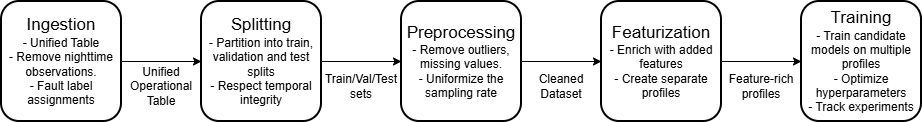
\includegraphics[width=\textwidth]{figures/chap3/pipeline-arch.png}
  \caption{Data pipeline architecture}
  \label{fig:pipeline}
\end{figure}

\begin{itemize}
    \item \textbf{Ingestion} converts raw sensor logs from a given field site into a unified operational table: acquisition streams recorded by heterogeneous systems at different sampling frequencies are joined and aligned, night-time observations are discarded, and the fault condition is assigned to a single shared label column. This conversion is the only stage that carries site-specific format knowledge; every downstream stage receives an identical schema and is fully insulated from the acquisition details of the source system.
    \item \textbf{Splitting} partitions the consolidated table into training, validation, and test sets according to a strict temporal grouping protocol. No sample-level transformation is performed at this stage; splitting is the gate at which evaluation integrity is established, and it must precede all subsequent stages that estimate statistics from the data.
    \item \textbf{Preprocessing} cleans the normal-class rows of the training partition through outlier removal (fault-labeled rows are exempt, as extreme values in those rows are expected fault signatures) and, for sites where the exploratory analysis identifies sustained temporal gaps in the field recording, tiered missing-value imputation, then estimates all cleaning statistics exclusively from that partition and applies them as fixed constants to validation and test.    
    \item \textbf{Feature engineering} transforms cleaned measurements into the representations consumed by the downstream models: named profiles specify which feature families are constructed, and a train-only selection stack eliminates redundant and low-relevance candidates before yielding the final feature matrices. The profile system makes this stage a controlled ablation instrument, isolating the contribution of each feature family across experiments.    
    \item \textbf{Model training} fits each candidate model on the feature-engineered partitions, restricts hyperparameter optimisation strictly to the training and validation partitions, and computes final metrics on the test partition exactly once after the winning configuration has been selected. All configurations, architectural choices, and evaluation results are tracked systematically, ensuring that every reported metric is traceable to a specific architectural state and data partition.
\end{itemize}


% \begin{figure}[H]
% \centering
% 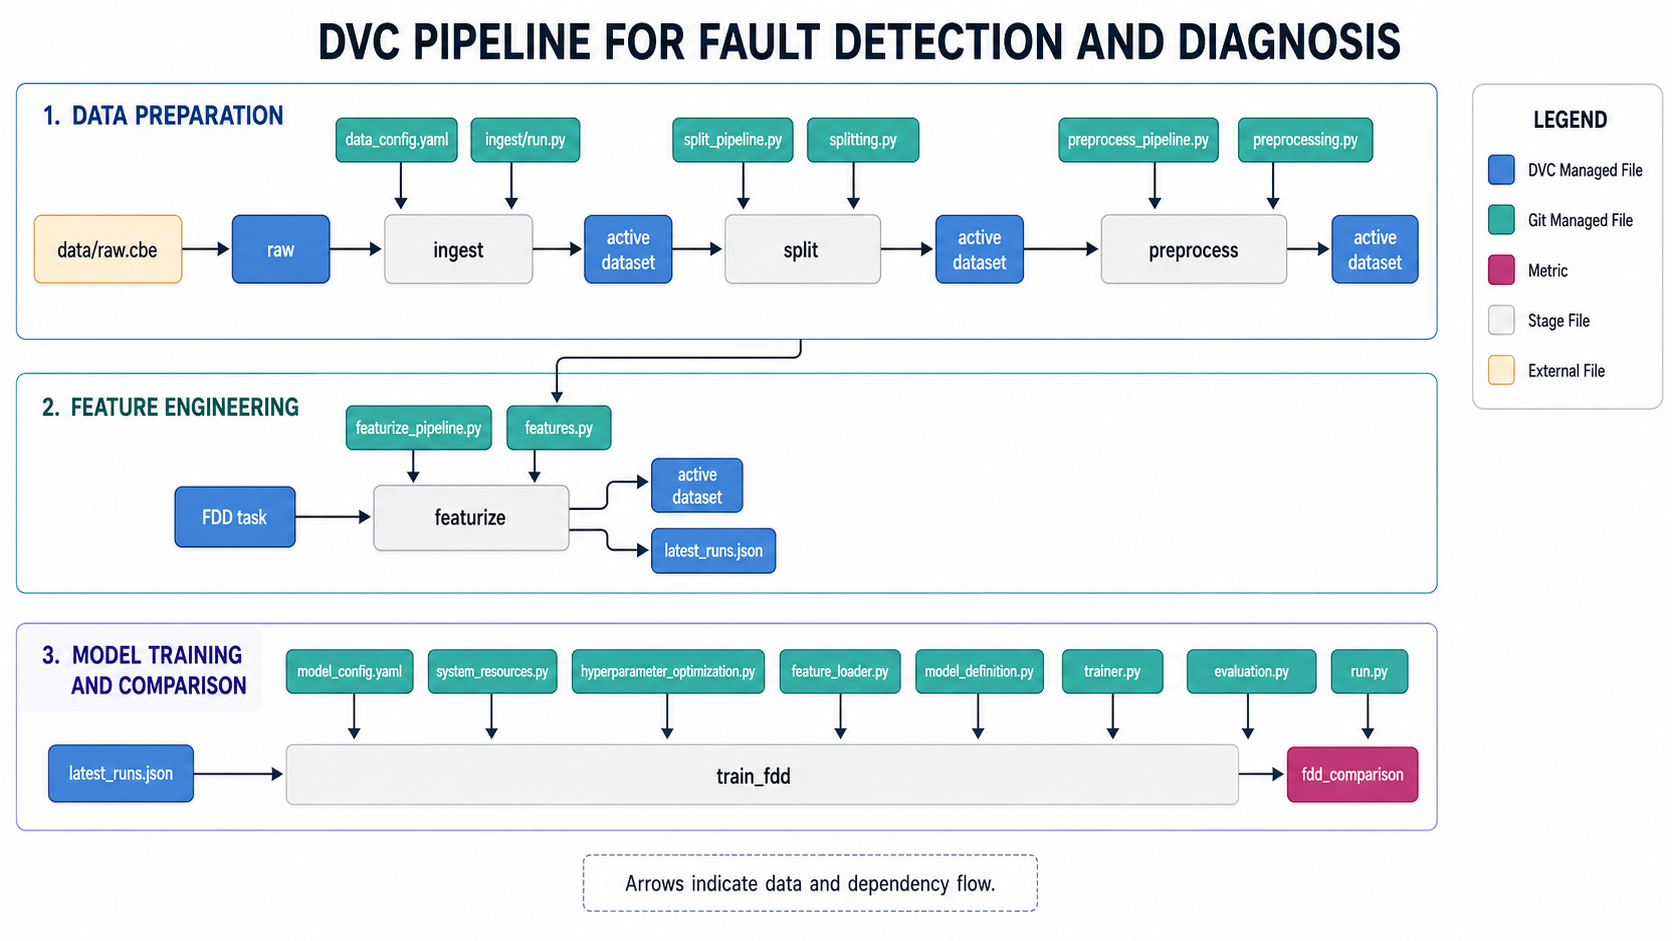
\includegraphics[width=\textwidth]{figures/dvc pipeline.png}
% \caption{Five-stage data pipeline from raw field recordings to model training and edge deployment.}
% \label{fig:pipeline}
% \end{figure}

% ────────────────────────────────────────────────────────────
\section{Conclusion}
% ────────────────────────────────────────────────────────────

This chapter specified the design of the proposed fault detection and diagnosis system for photovoltaic installations, from the high-level system architecture to the data and modeling foundations required for reliable operation on field measurements. Two complementary datasets were selected to support both development and generalization assessment: Costa as the primary multi-fault classification benchmark and La~Réunion as a shading-focused field benchmark under long-term operating variability.

The exploratory audit established the concrete constraints that drive the remainder of the pipeline design. In particular, production-regime filtering prevents artificial class separability from night-time zeros, label-aware cleaning preserves fault signatures while suppressing true sensor glitches, and time dependence is treated as a first-class concern through temporally coherent episode definitions and leakage-preventing partition boundaries. These findings also motivate the feature design philosophy: engineered representations should encode physically meaningful invariants (irradiance normalization, inter-string imbalance, temperature correction, and temporal derivatives) while remaining robust to regime shifts and collinearity.

Finally, the overall pipeline is defined as a staged DAG that separates ingestion, splitting, preprocessing, feature engineering, and model training. This modular structure makes evaluation integrity enforceable at a clear boundary, supports controlled ablations, and enables the same design to be applied consistently across heterogeneous field sites. The next chapter describes how these design requirements are implemented and operationalized in the experimental pipeline.

